\chapter{FESDData Appendix}

This appendix contains graphs which were not included in the main body of the thesis.

\section{Distribution of the number of joints with an error}

Each problem set, except the joint problem set, is an abstraction from the base data which combines different areas of the pose into separate objects. A threshold is used to determine whether an area is considered as faulty based on the number of joints that are faulty in the pose. To determine this threshold the distribution of joints with errors is calculated for each of the problem areas over all the data and the 50th percentile is picked as the threshold.

\paragraph{Full Body problem set}

The results of the full body problem set can be seen in Figure \ref{fig:dist_jt_epp}. The threshold is at two errors, i.e. if more than two joints in the whole body are faulty, the whole body is considered as faulty.

\begin{figure}[ht]
  \centering
  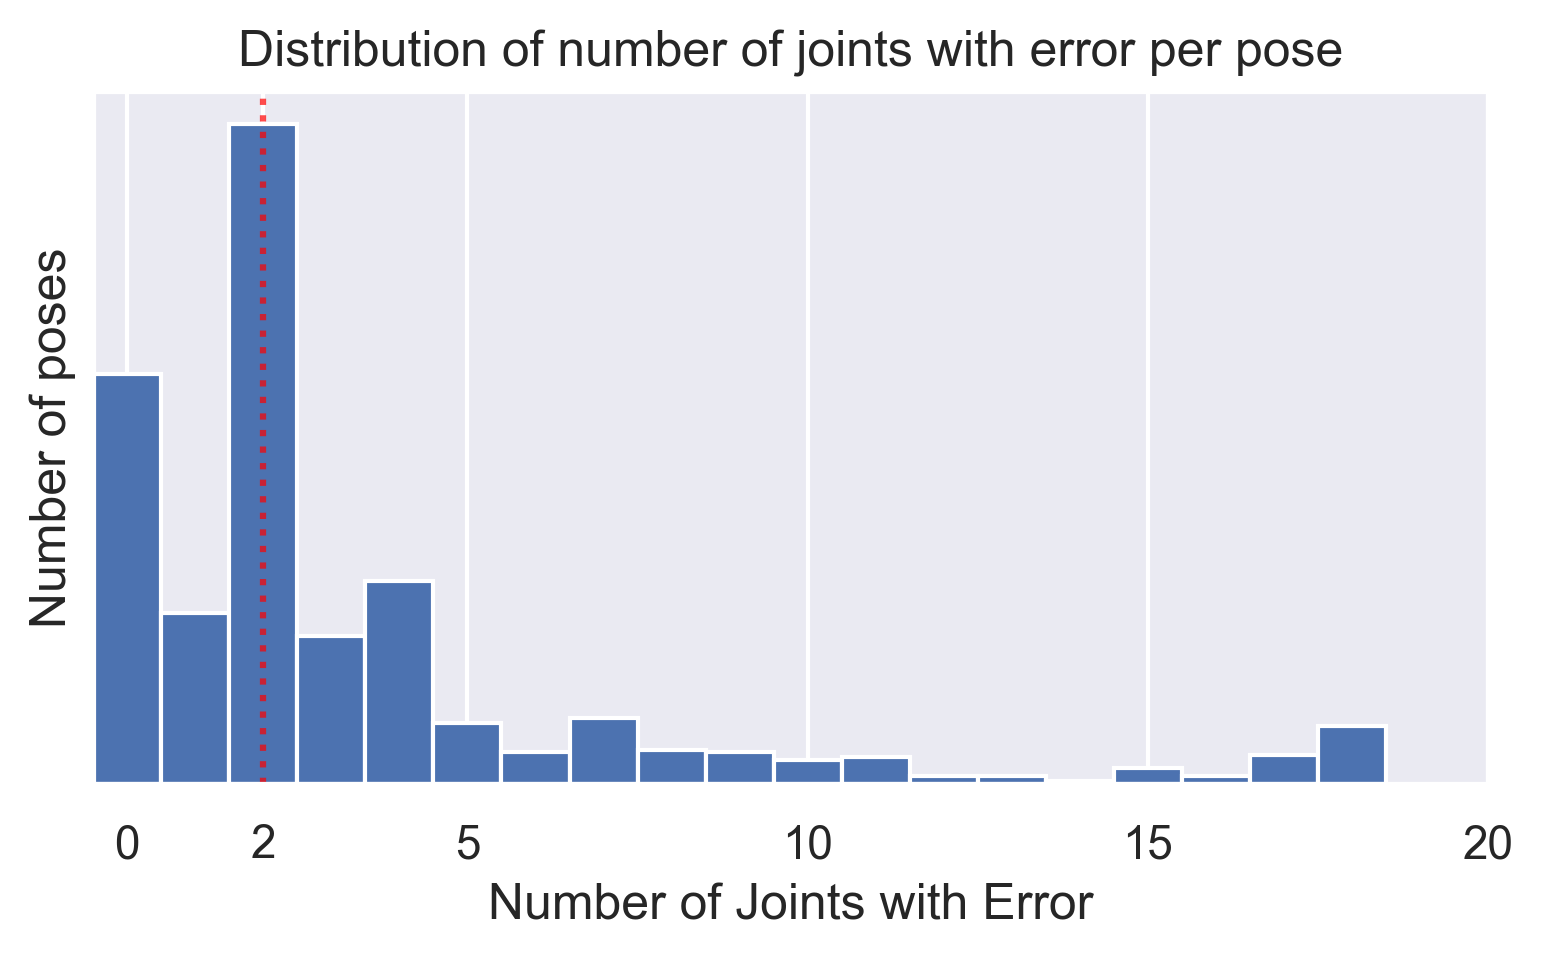
\includegraphics[width=0.8\textwidth]{figures/Data/joint_errors_per_pose/distribution_of_joint_errors_per_pose.png}
  \caption[Number of Joints with error]{The distribution of the number of joints with errors in each frame.}
  \label{fig:dist_jt_epp}
\end{figure}

\paragraph{Half Body problem set}

The distribution of joints with errors for both the lower and upper body can be seen in figure \ref{fig:dist_bh_epp}. If one joint in the upper body or more than two joints in the lower body are considered as faulty, the upper or lower body is considered as faulty respectively.

\begin{figure}[ht]
  \centering
  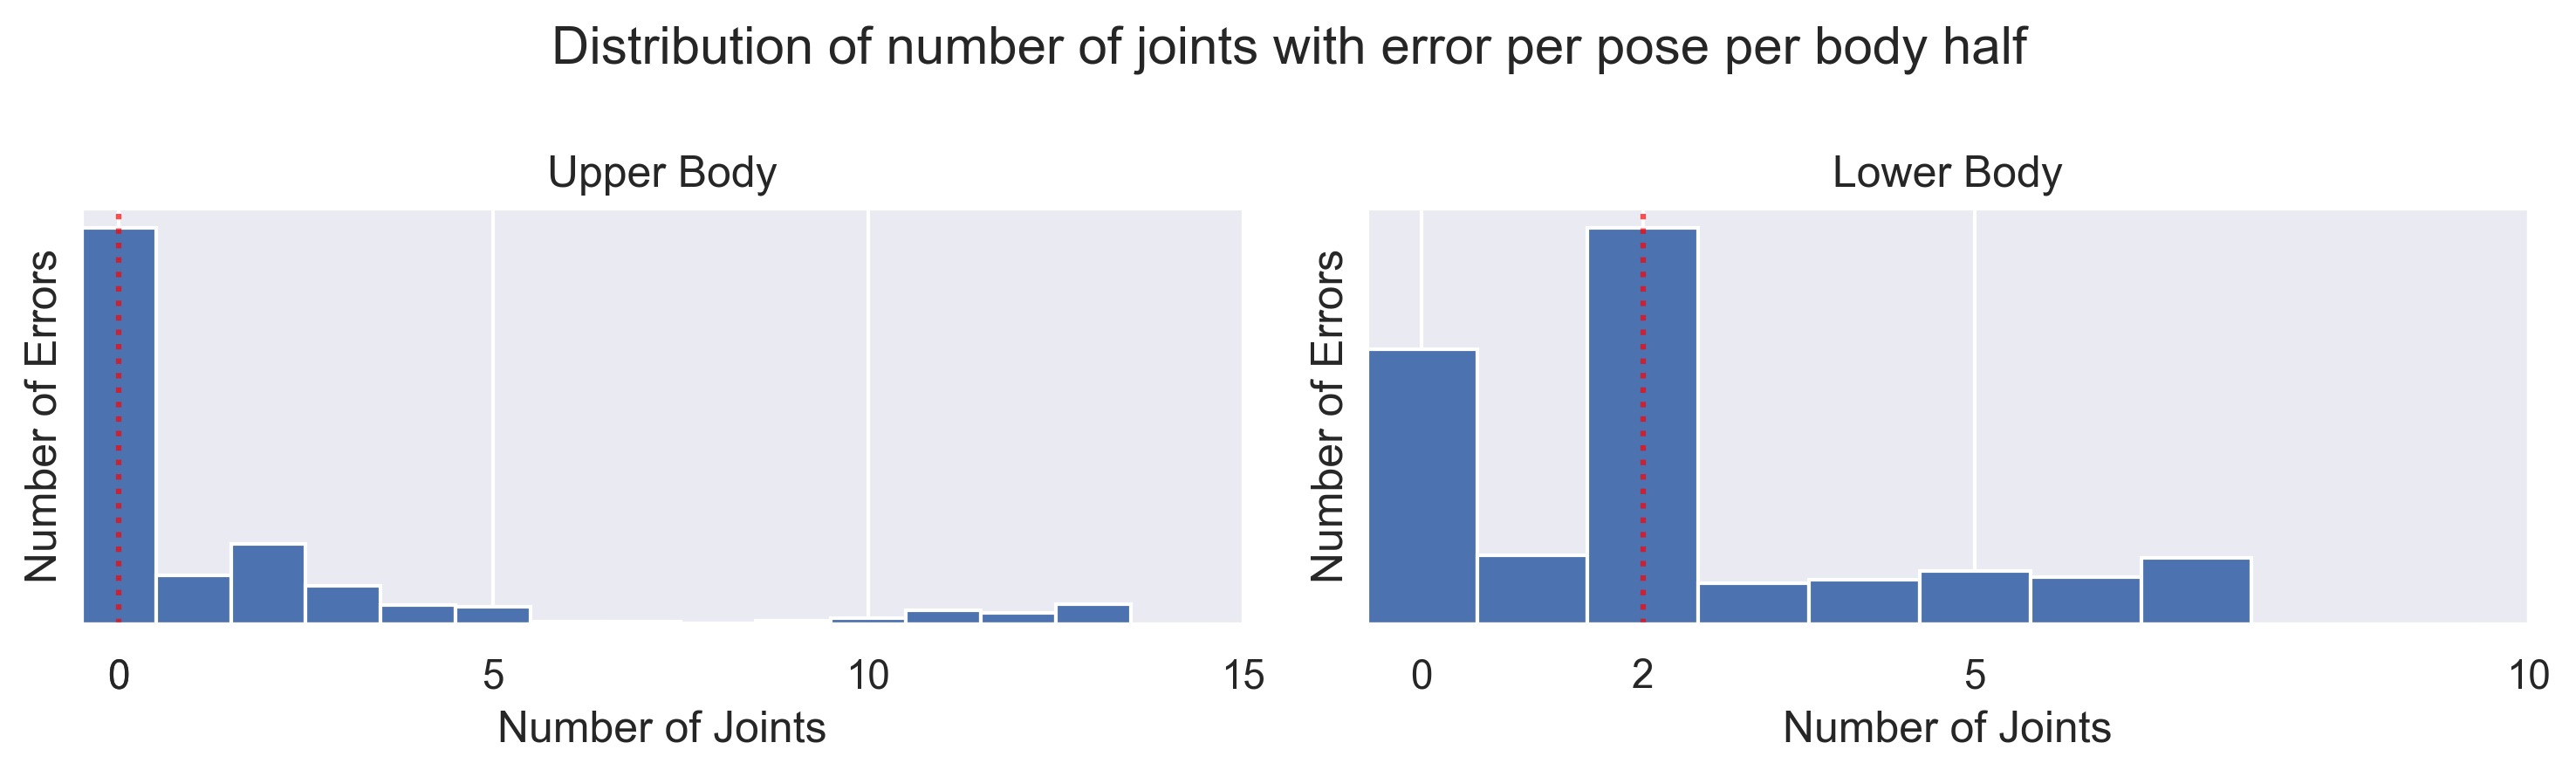
\includegraphics[width=0.8\textwidth]{figures/Data/joint_errors_per_pose/distribution_of_joint_errors_per_pose_per_body_half.png}
  \caption[Number of Joints with error per body half]{The distribution of the number of joints with errors in each frame per body half.}
  \label{fig:dist_bh_epp}
\end{figure}

\paragraph{Body parts problem set}

The left and right Legs require two or more faulty joints. Whereas all other body parts require only one or more errors to be considered as faulty. 

\begin{figure}[ht]
  \centering
  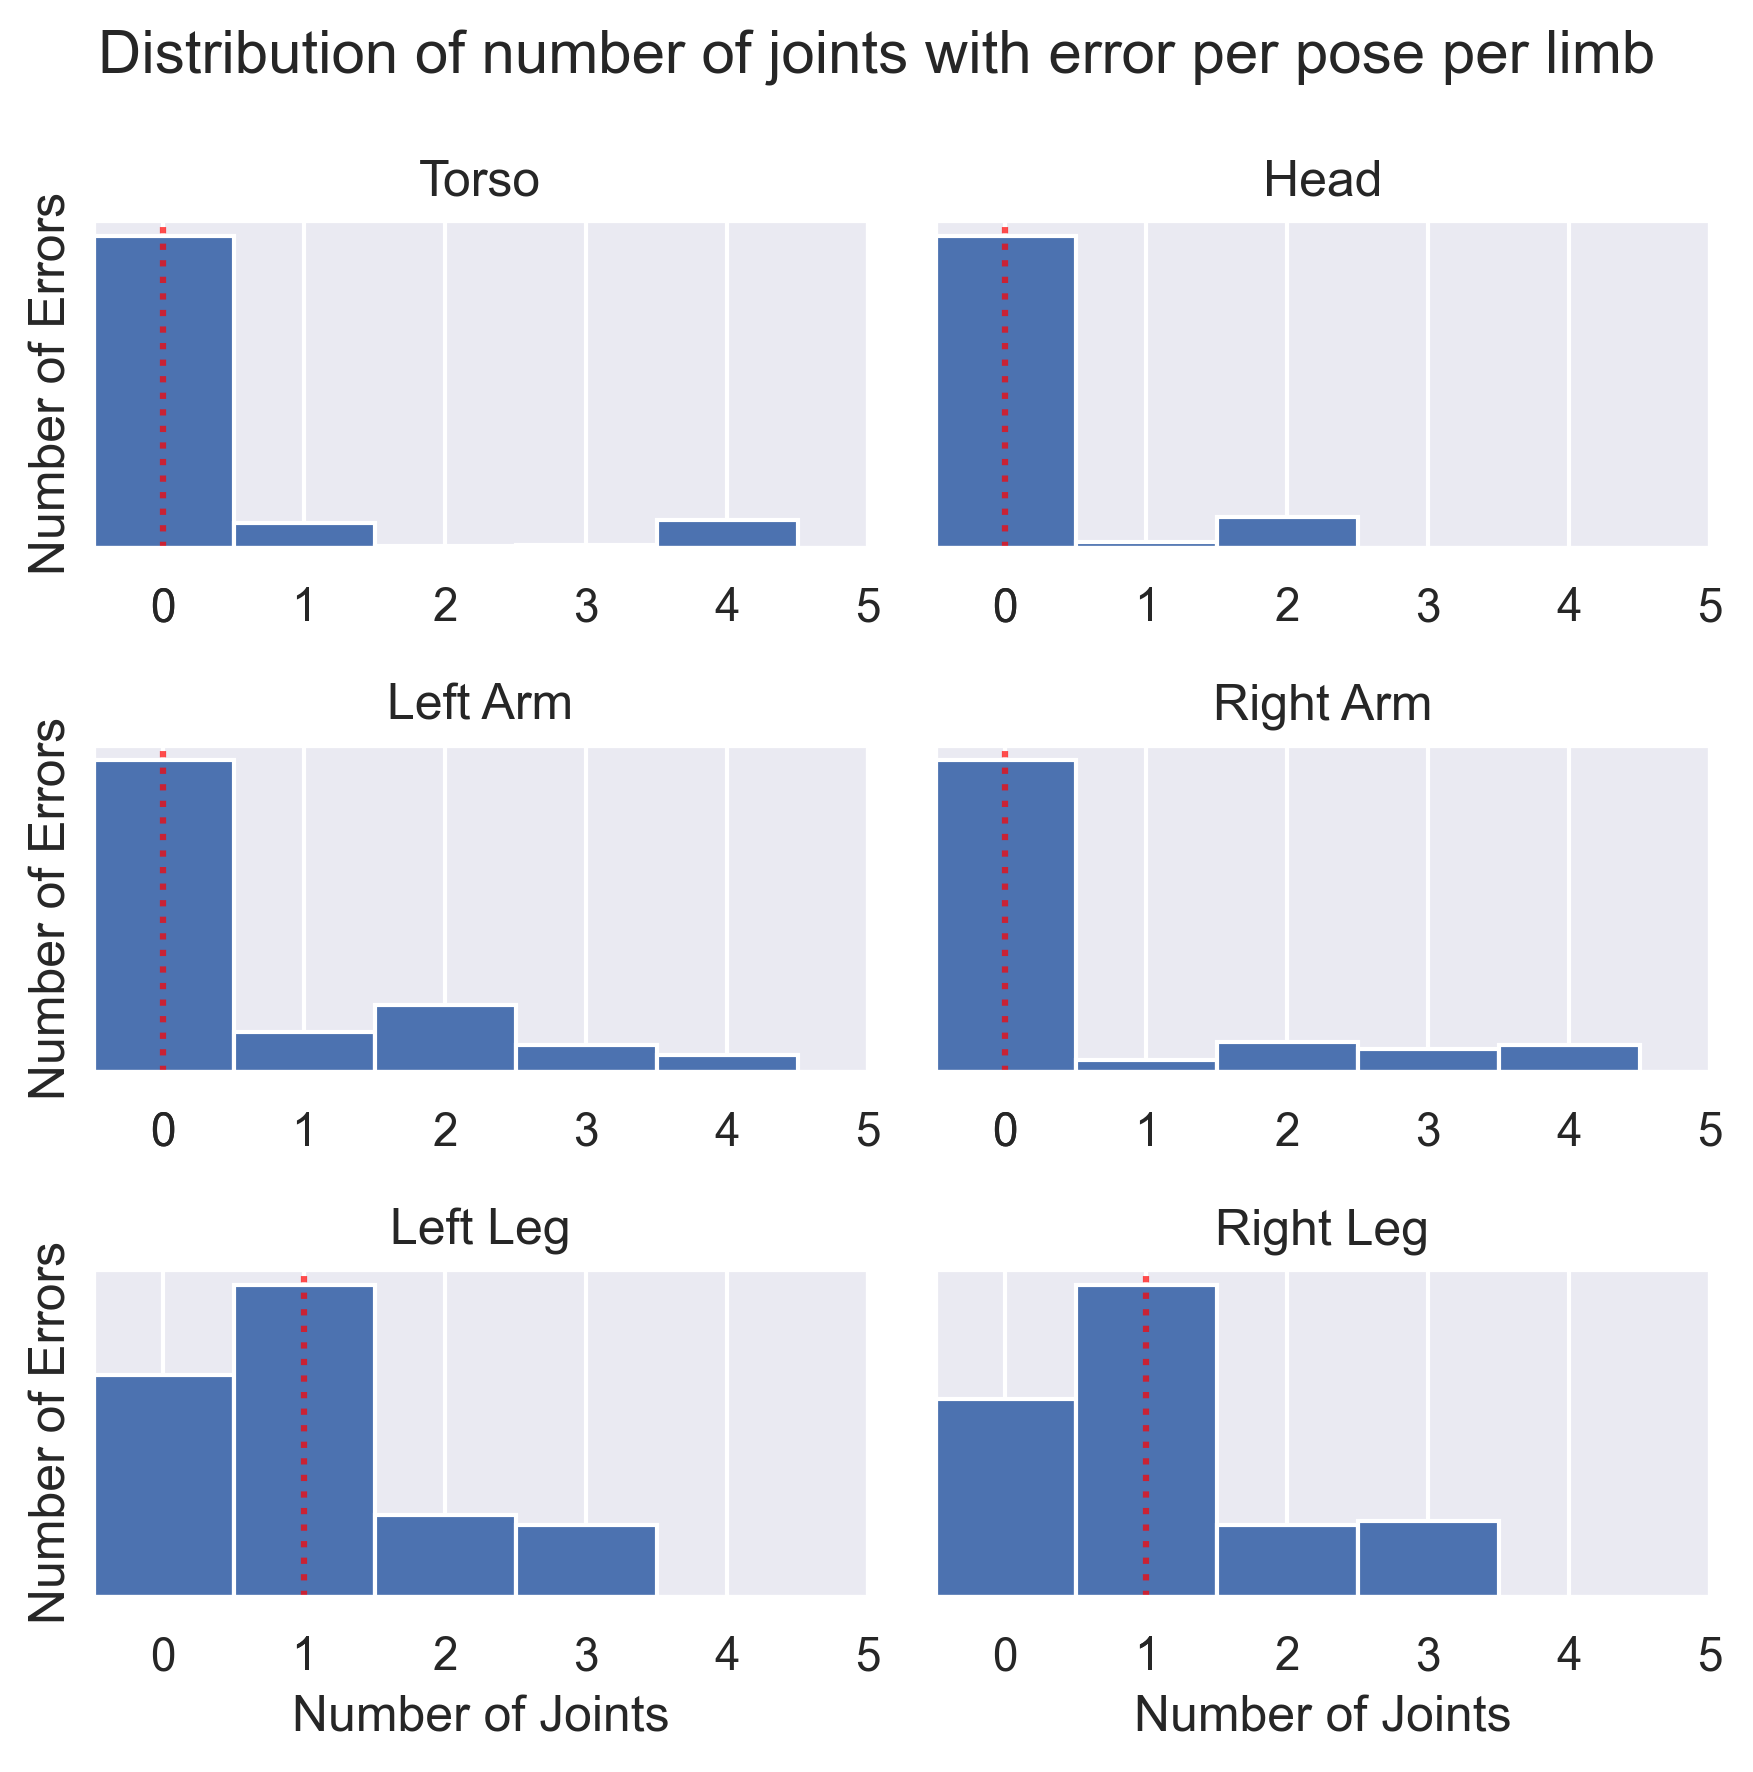
\includegraphics[width=0.6\textwidth]{figures/Data/joint_errors_per_pose/distribution_of_joint_errors_per_pose_per_body_part.png}
  \caption[Number of Joints with error per body part]{The distribution of the number of joints with errors in each frame per body part.}
  \label{fig:dist_lb_epp}
\end{figure}

\section{Distribution of Errors}

This section contains the different distributions of errors for each of the problem sets.

\paragraph{Full Body}

Figure \ref{fig:fb_diff_dist} gives an overview of the error distribution by the difficulty of the exercise. The figure indicates that the difficulty of the exercise directly influences the percentage of errors that occur.

\begin{figure}[ht]
  \centering
  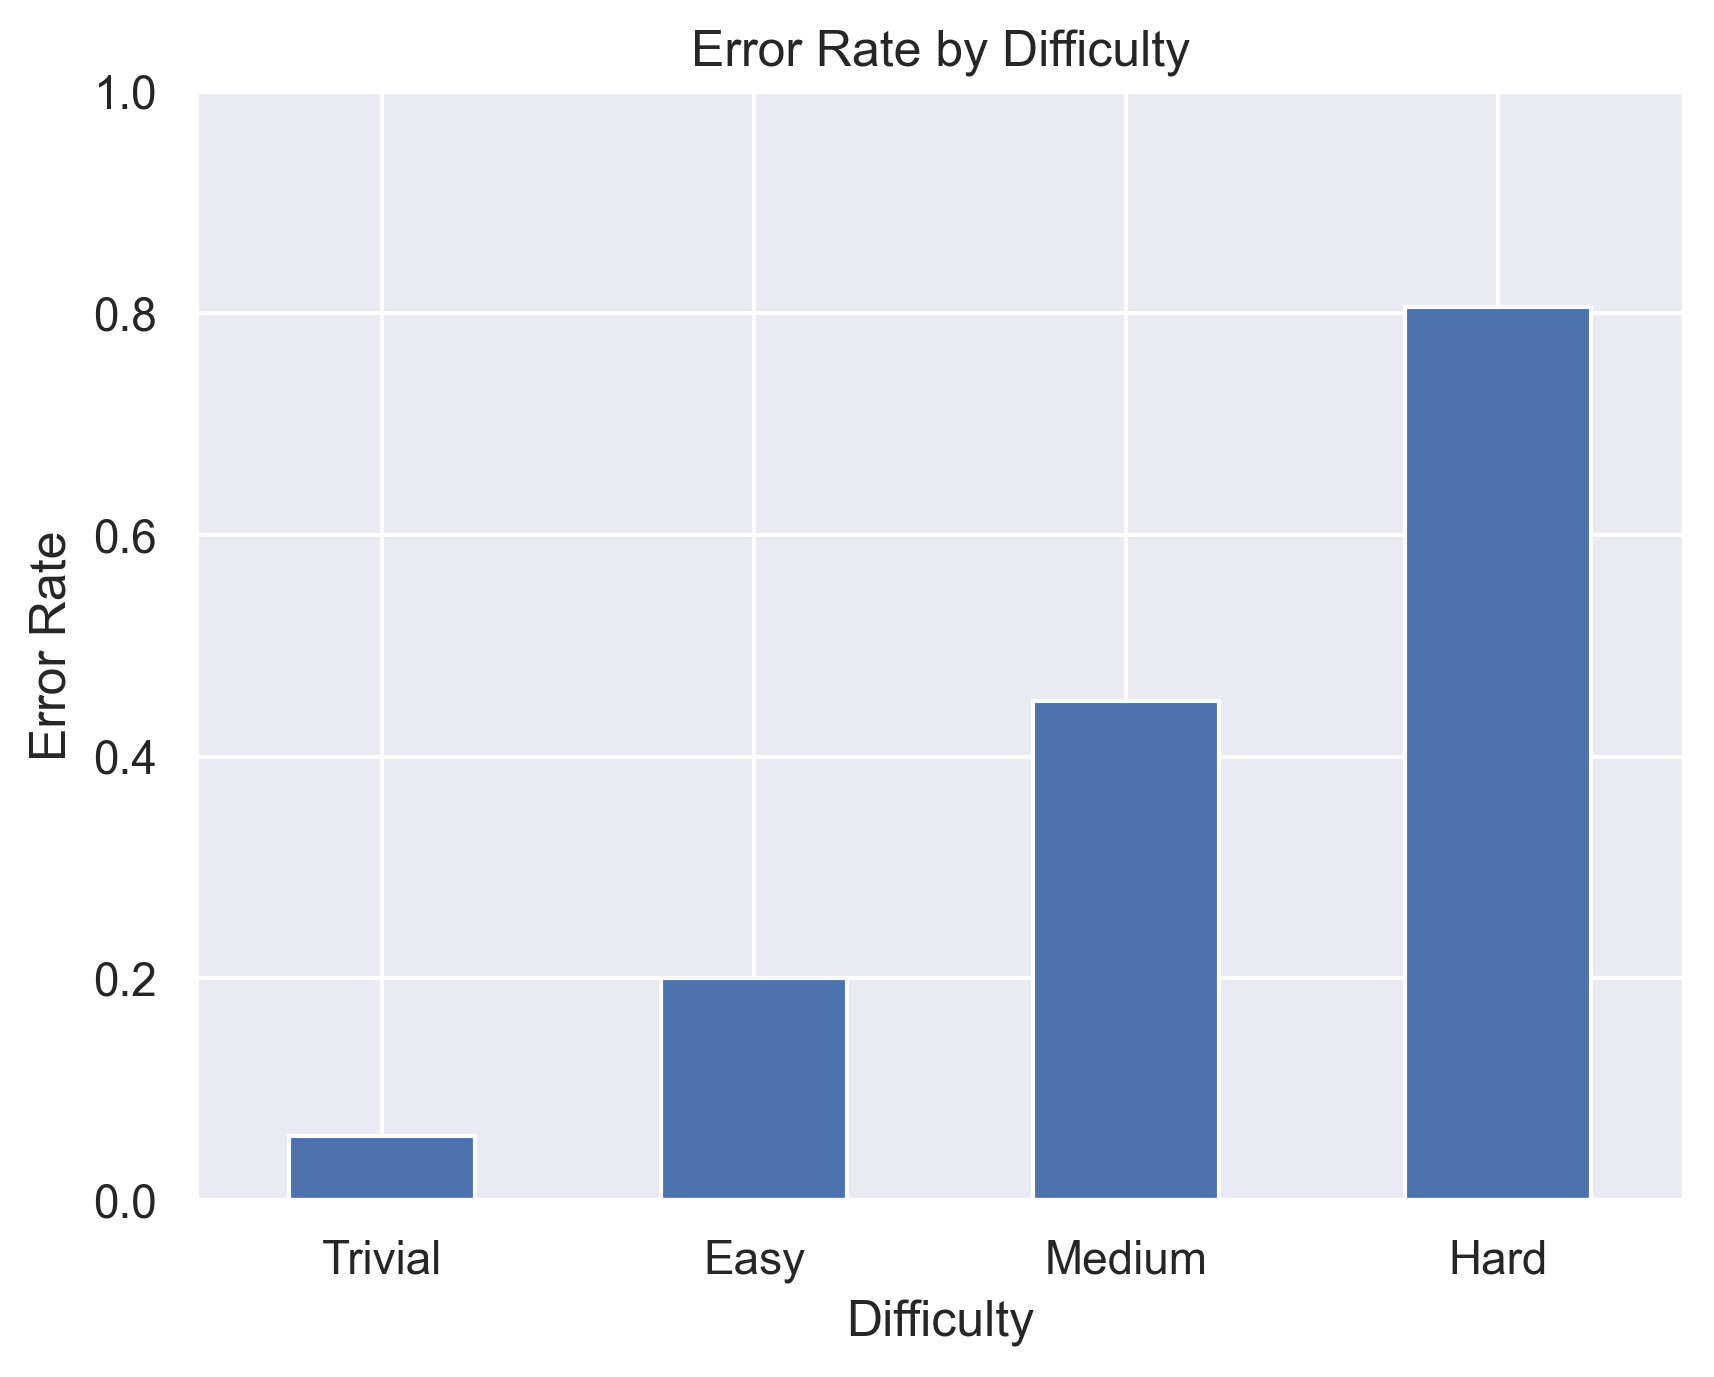
\includegraphics[width=0.8\textwidth]{figures/Data/dist_full_body/Error_Rate_by_Difficulty.png}
  \caption[Error Distribution of the Full Body by difficulty]{The distribution of Errors of the full body problem set by difficulty.}
  \label{fig:fb_diff_dist}
\end{figure}

\paragraph{Half Body}

The distribution of errors by difficulty for the half body problem set can be seen in figure \ref{fig:hb_diff_dist}. Easy exercises seem to be less error-prone when grouping the joints into body halves. This might be caused by the error threshold that was set before.

\begin{figure}[ht]
  \centering
  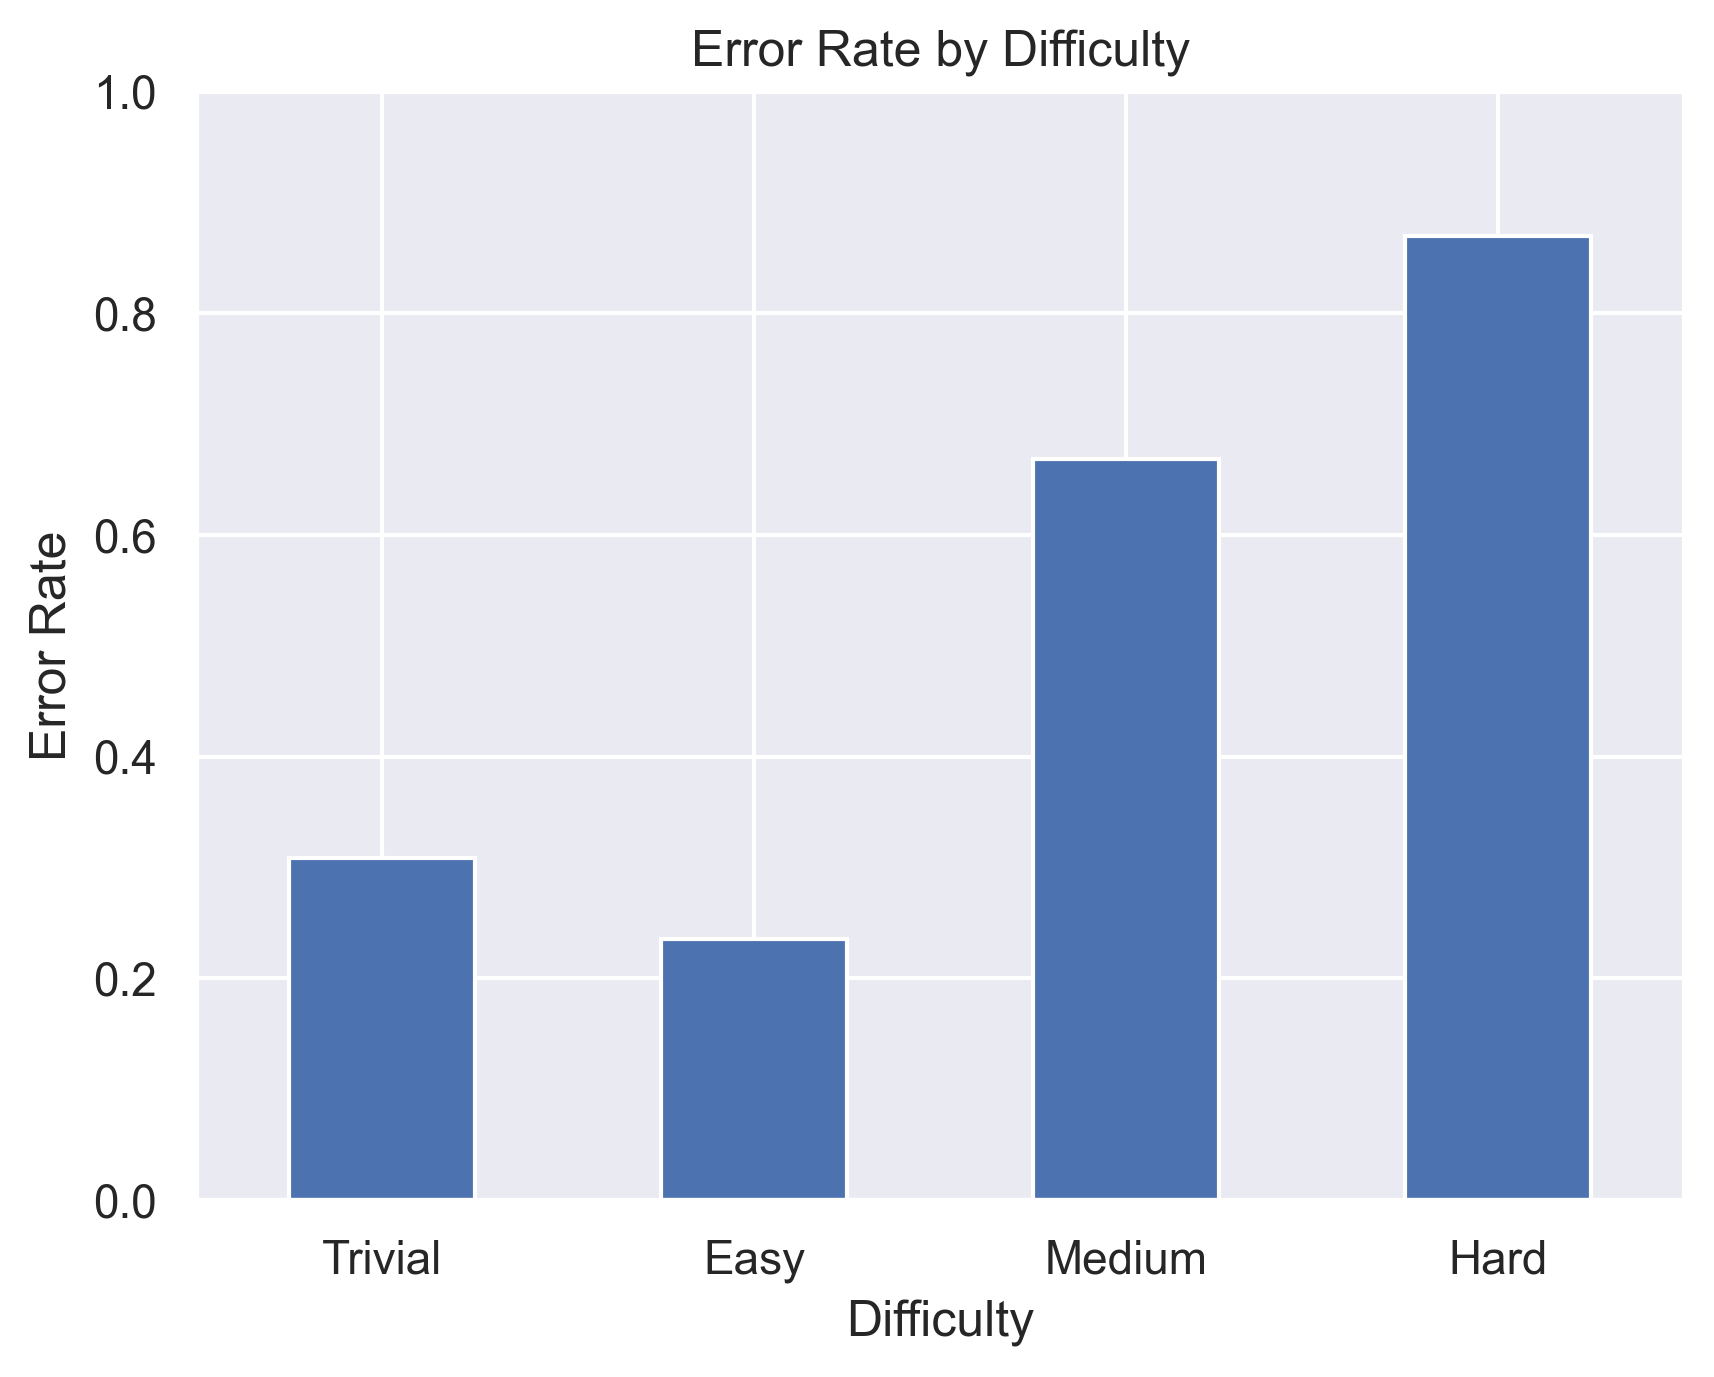
\includegraphics[width=0.8\textwidth]{figures/Data/dist_half_body/Error_Rate_by_Difficulty.png}
  \caption[Error Distribution of the Half Body by difficulty]{The distribution of Errors of the half body problem set by difficulty.}
  \label{fig:hb_diff_dist}
\end{figure}

\paragraph{Body parts}

The distribution of errors by difficulty can be seen in figure \ref{fig:lb_diff_dist}. A less distinct distribution of errors can be seen when grouping the joints into body parts. Only a very small amount of errors occur during trivial exercises. This might be caused by the error threshold that was set before. The majority of errors occurring during trivial exercises are caused by a single faulty joint in the ankle. In Figure \ref{fig:dist_lb_epp} it is shown that the legs have an error threshold of two faulty joints. This means that the legs are considered faulty if there are more than two faulty joints. The ankle is the only joint that is faulty in trivial exercises. This means that the legs are not considered faulty.

\begin{figure}[ht]
  \centering
  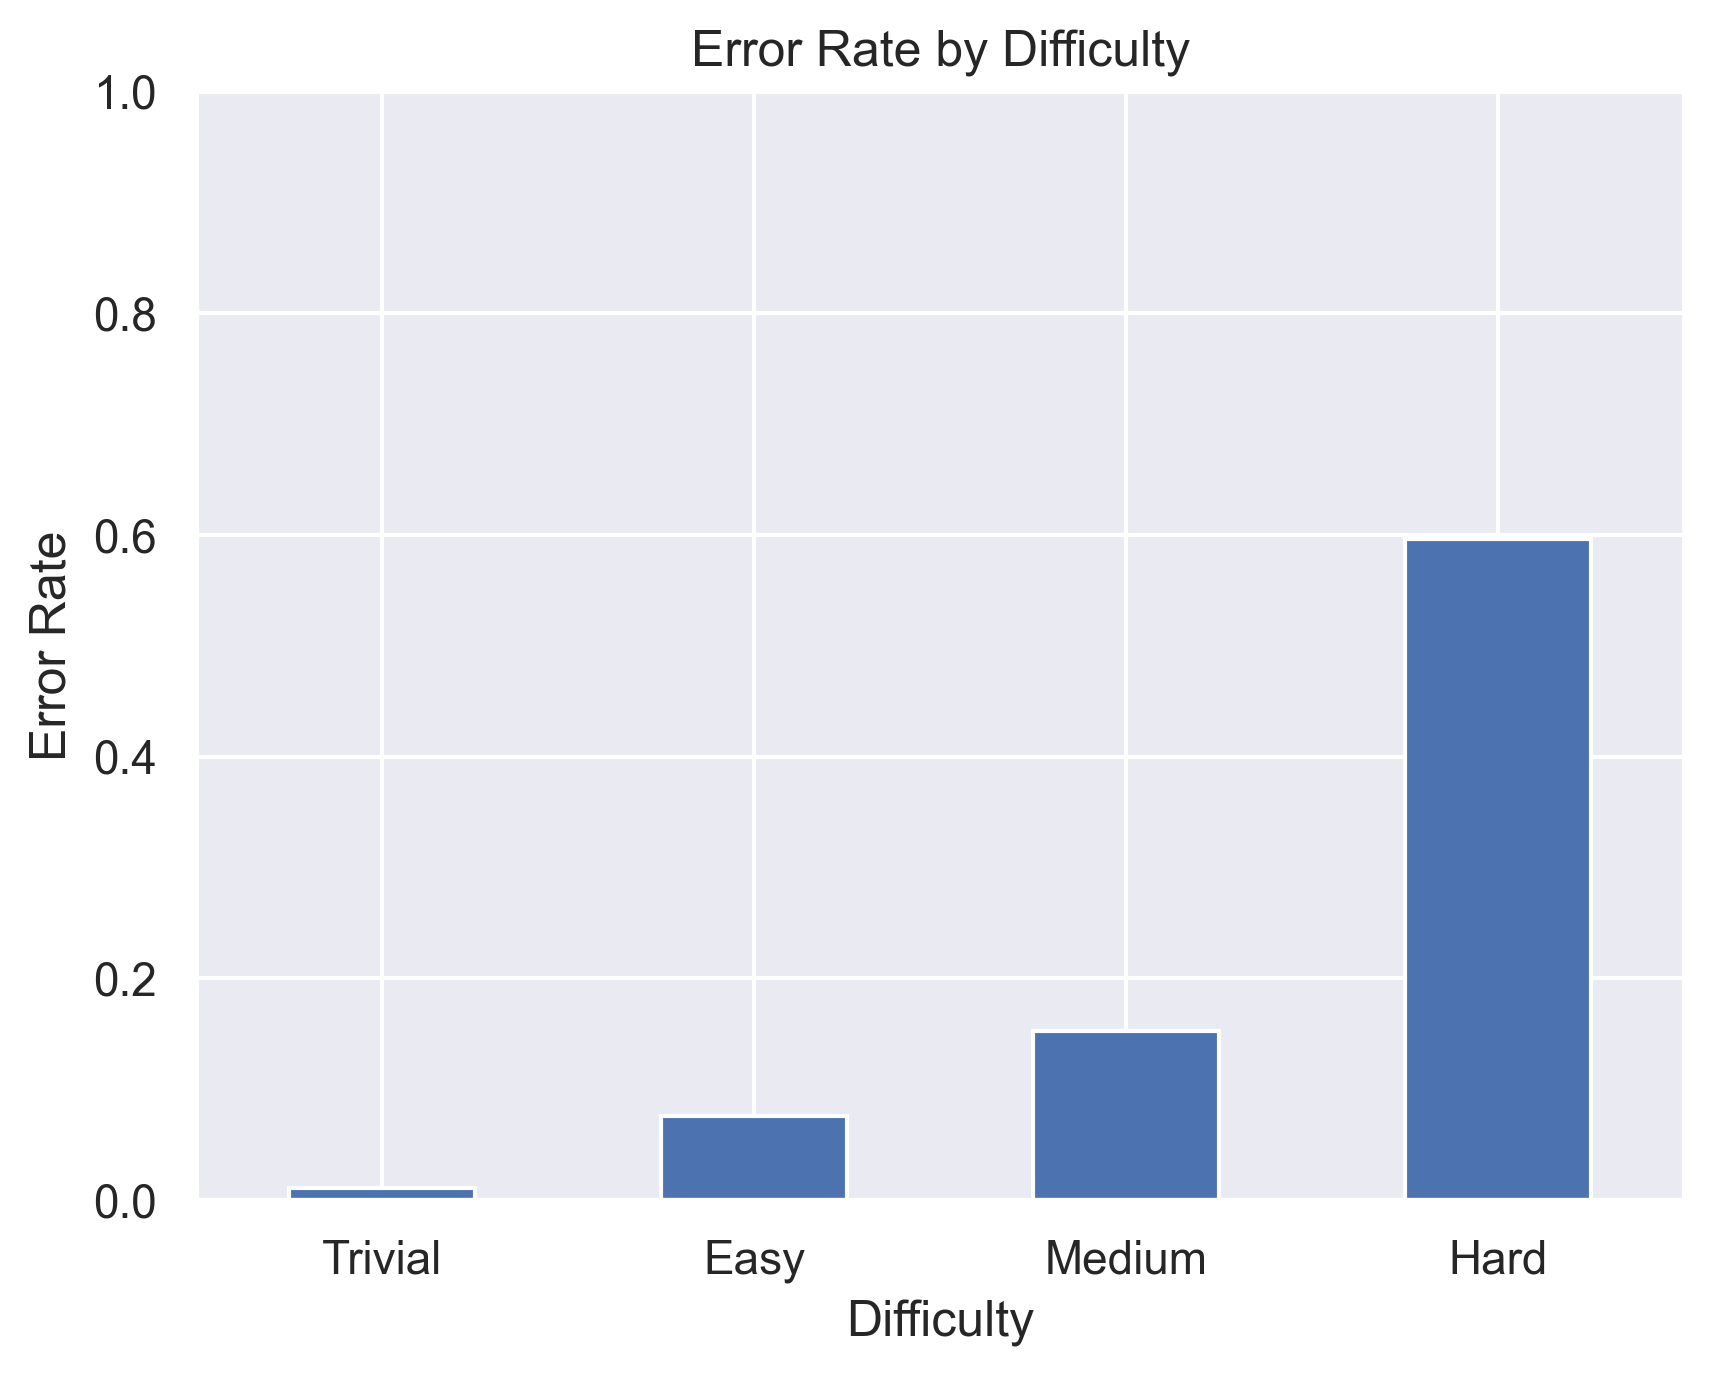
\includegraphics[width=0.8\textwidth]{figures/Data/dist_limbs/Error_Rate_by_Difficulty.png}
  \caption[Error Distribution of the body parts by difficulty]{The distribution of Errors of the half-body problem set by difficulty.}
  \label{fig:lb_diff_dist}
\end{figure}

\paragraph{Joints}

In medium exercises, the majority of errors that occur for the joints problem set, occur due to missing joints, rather than joints which are in the wrong position. This is shown in figure \ref{fig:jt_pie_diff}.

A clear distinction between error-prone and stable joints can be seen in figure \ref{fig:jt_pie_joint}. While in the majority of cases ($72.3\%$) the right ankle is faulty only $4.9\%$ of the left shoulder is faulty. Furthermore, the left and right ankles have a significant number of missing joints, contrary to the other joints, which have a more balanced distribution of error classes. This might be caused by occlusion or a cutoff from the image or a confidence which is too low and therefore discarded by Nuitrack.

\begin{figure}[ht]
  \centering
  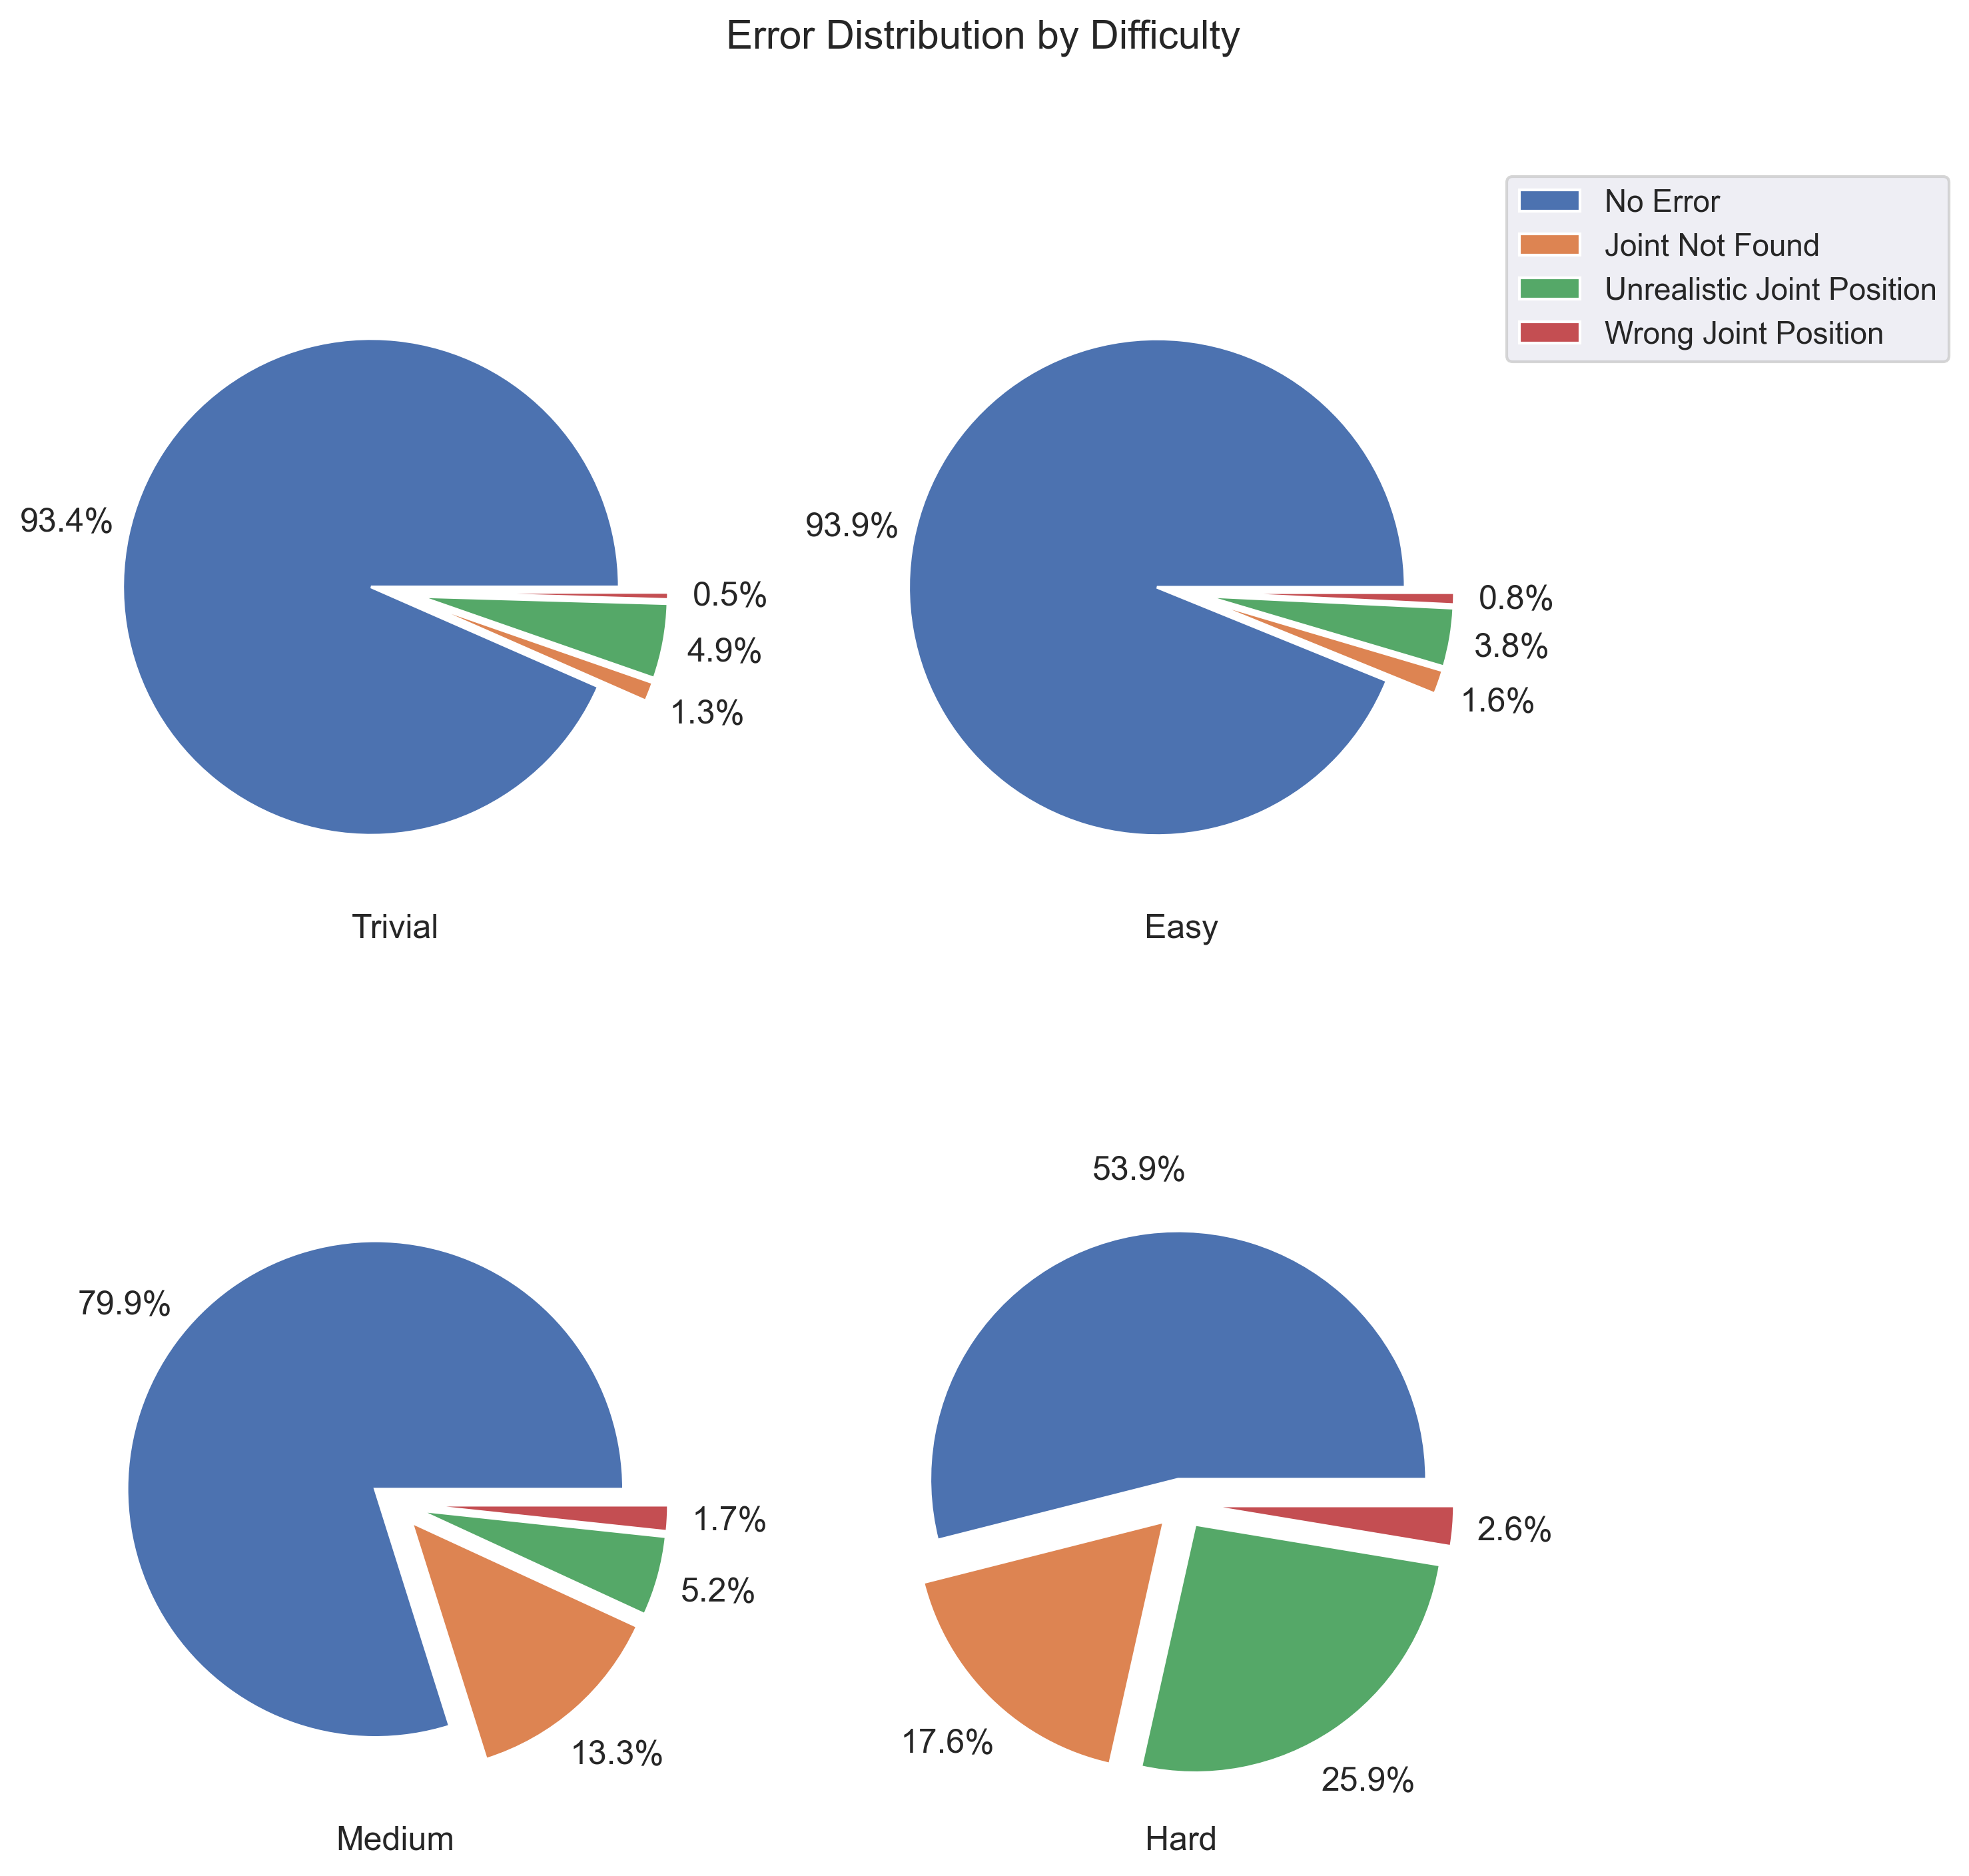
\includegraphics[width=0.8\textwidth]{figures/Data/dist_joints/Error_Distribution_by_Difficulty.png}
  \caption[Error Distribution for each error class by difficulty]{The distribution of each error class grouped by difficulty.}
  \label{fig:jt_pie_diff}
\end{figure}

\begin{figure}[ht]
  \centering
  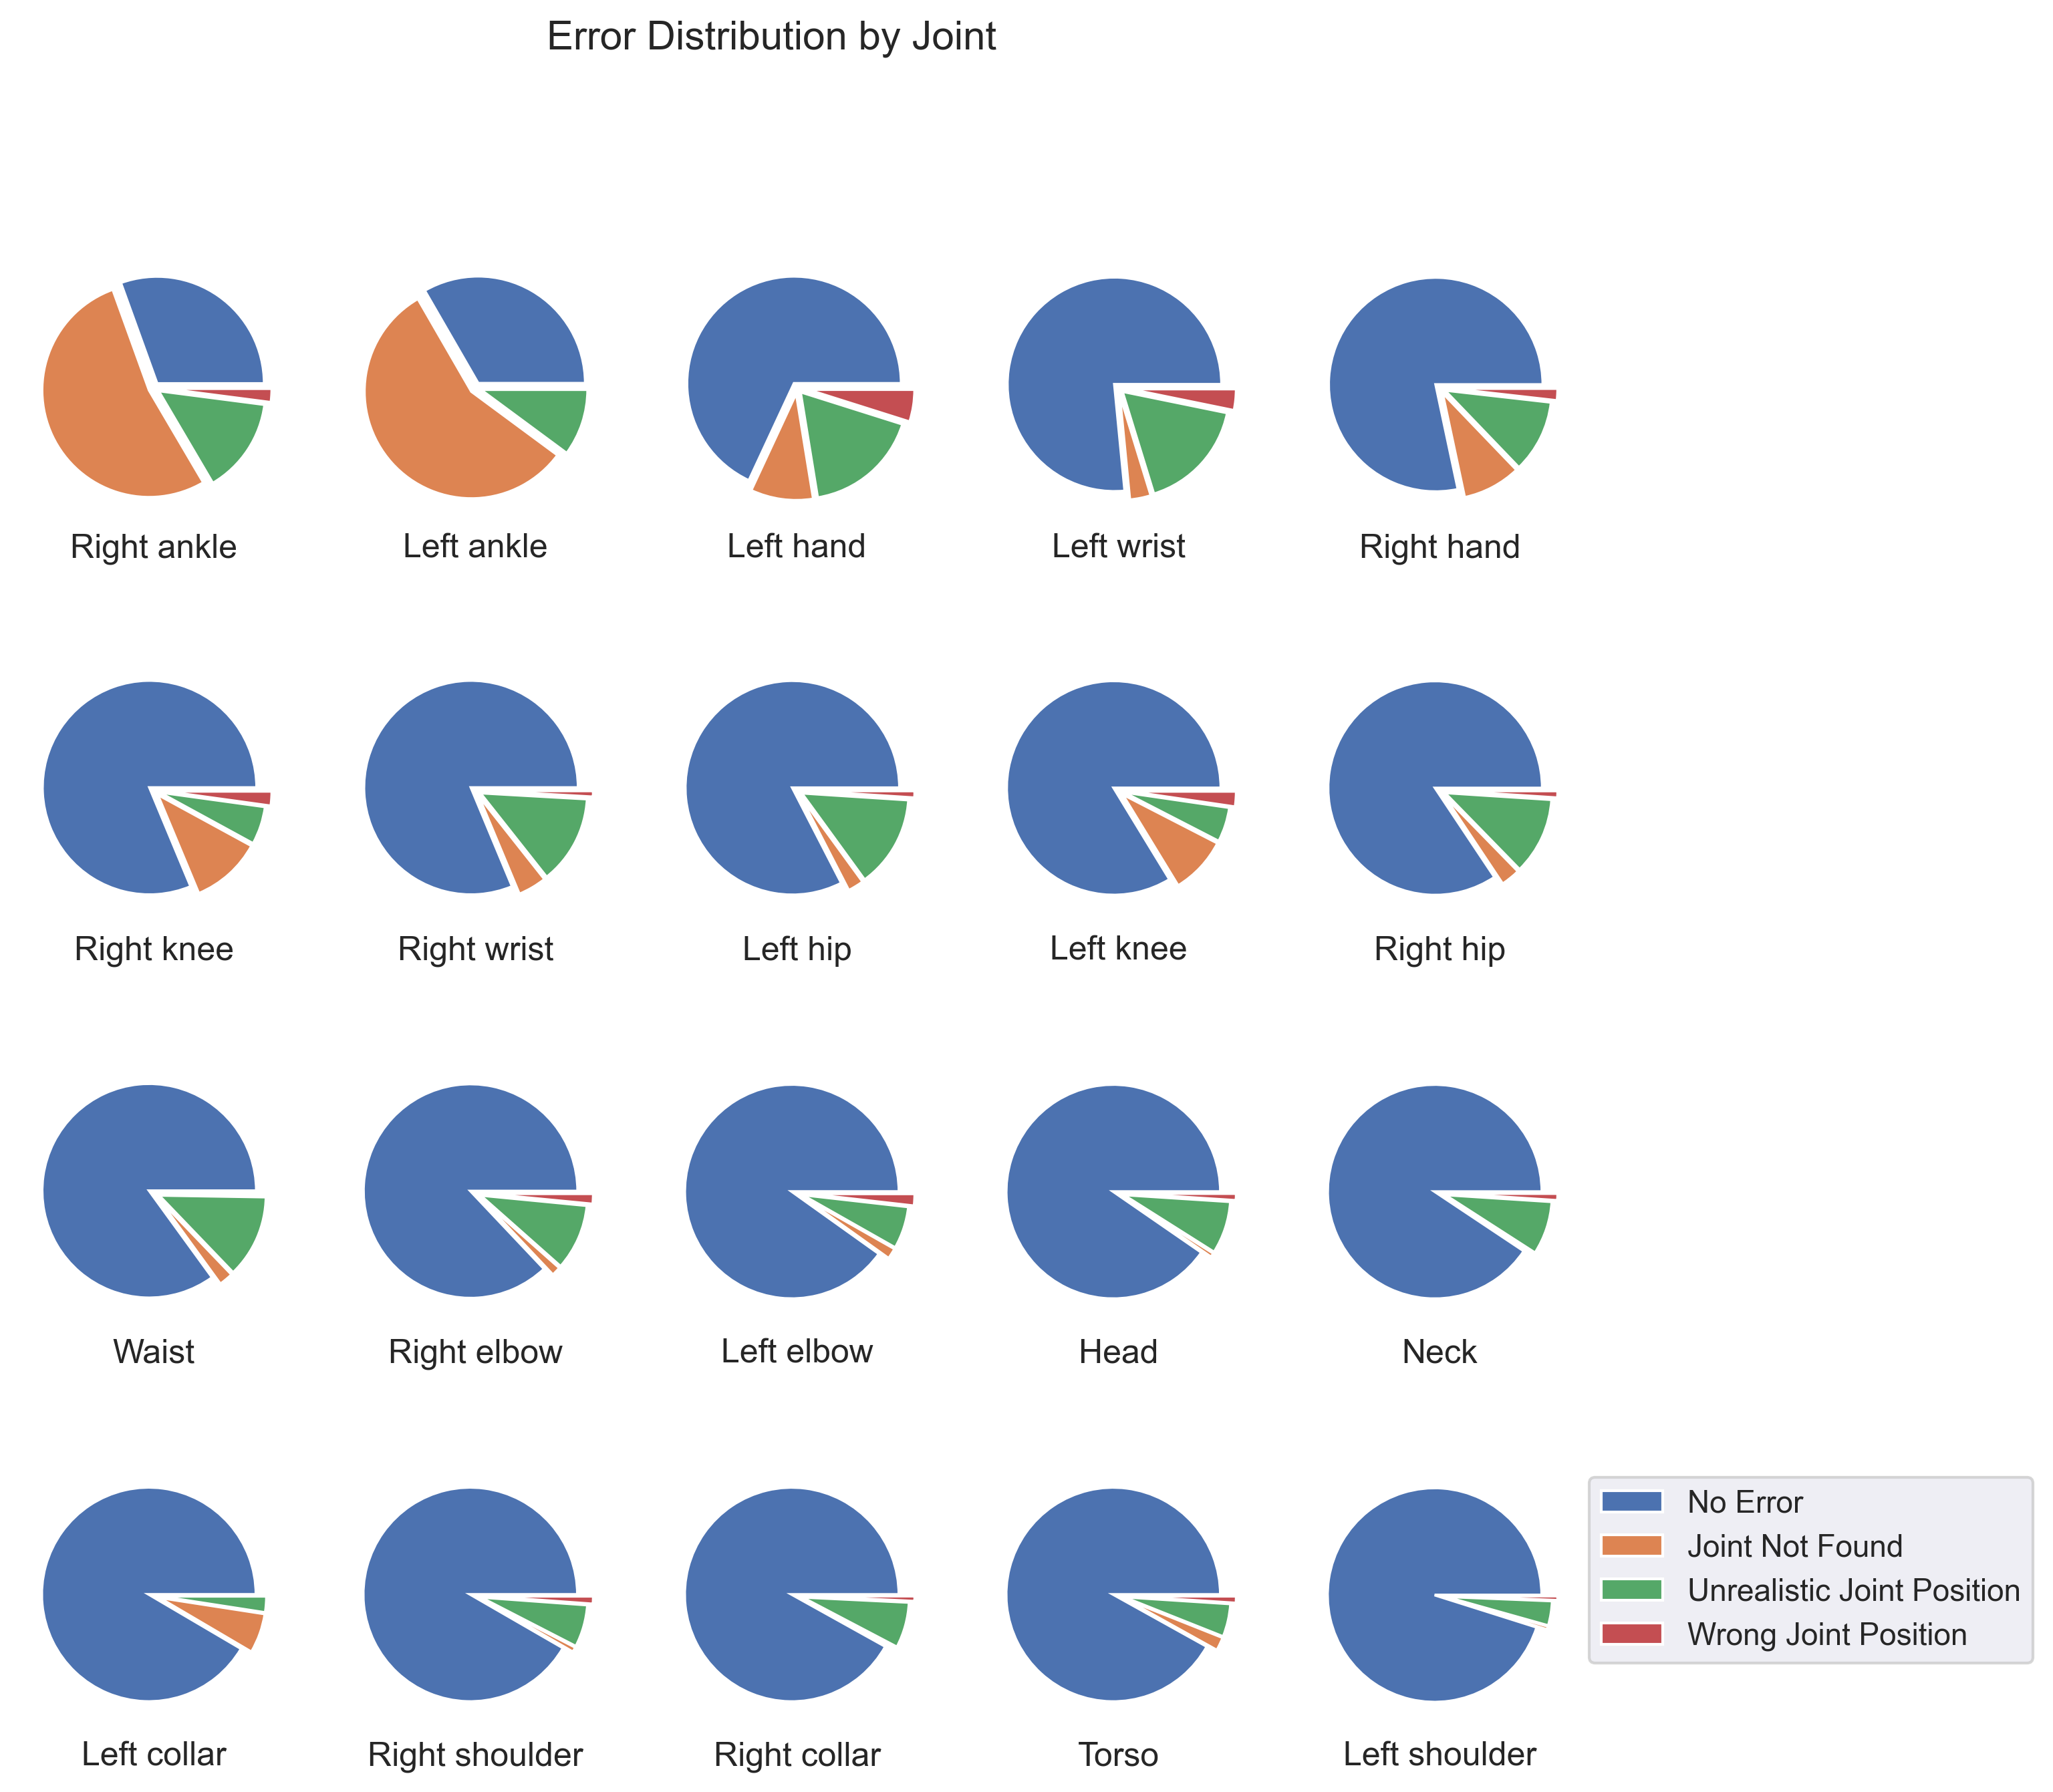
\includegraphics[width=0.8\textwidth]{figures/Data/dist_joints/Error_Distribution_by_Joint.png}
  \caption[Error Distribution for each error class by joint]{The distribution of each error class grouped by joint.}
  \label{fig:jt_pie_joint}
\end{figure}

\begin{figure}[ht]
  \centering
  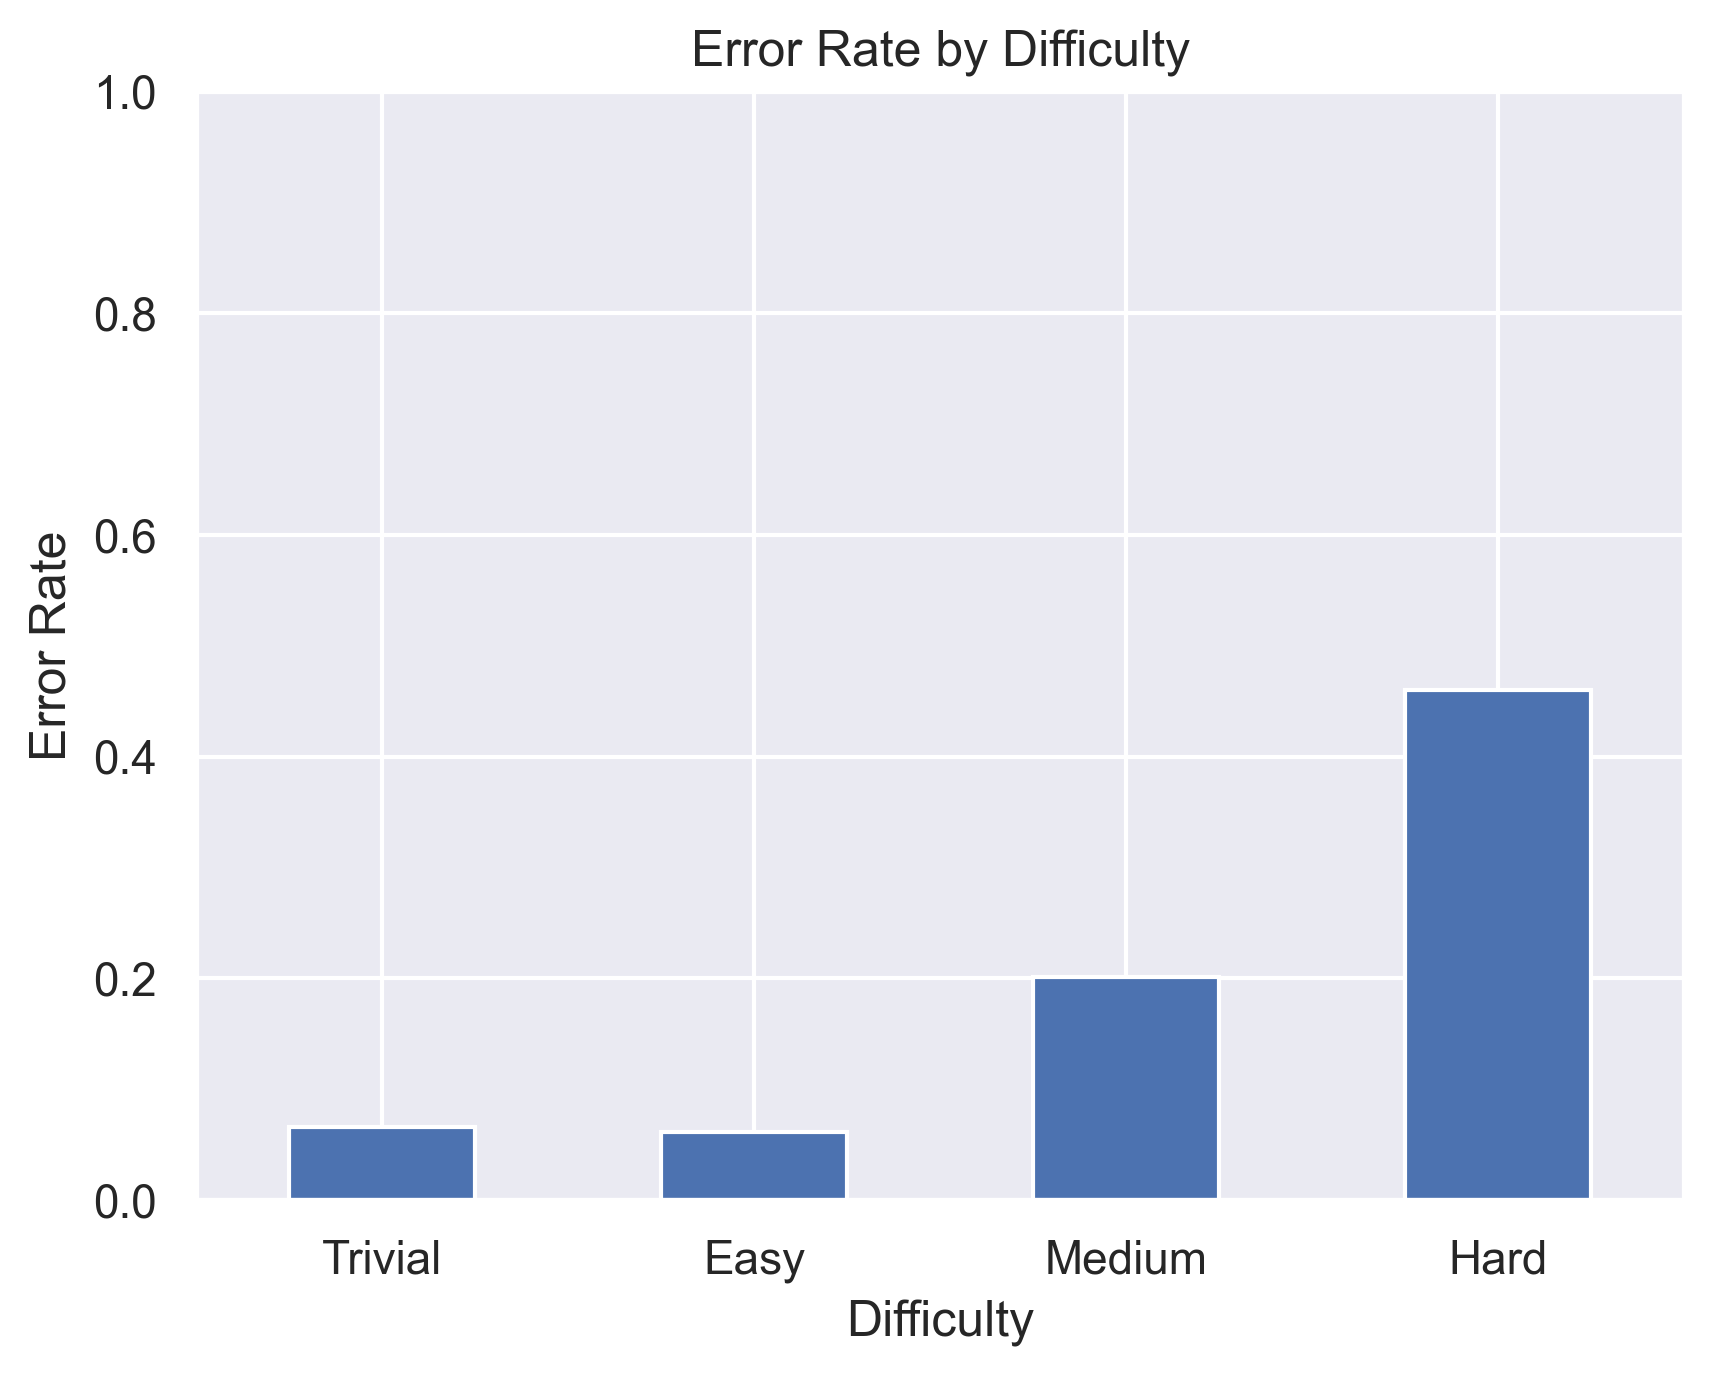
\includegraphics[width=0.8\textwidth]{figures/Data/dist_joints/Error_Rate_by_Difficulty.png}
  \caption[Error Distribution of the joints by difficulty]{The distribution of Errors of the joint problem set by difficulty.}
  \label{fig:jt_diff_dist}
\end{figure}
